\documentclass[12pt, a4paper]{article}
\usepackage[backend=biber,style=ieee,sorting=nty]{biblatex}
\usepackage{blindtext}
%\usepackage{cite}
%\usepackage{draftwatermark}
\usepackage{enumitem}
\usepackage{framed}
\usepackage{soul}
\usepackage{tikz,tkz-tab,amsmath}
\usepackage{wrapfig}
\usepackage{xcolor}
\usepackage{typed-checklist}
\definecolor{shadecolor}{gray}{0.9}
\newtheorem{question}{Q\ignorespaces}
%\SetWatermarkText{DRAFT}
%\SetWatermarkScale{5}
%\SetWatermarkColor[gray]{0.7}

\setlength{\oddsidemargin}{0.5cm}
\setlength{\evensidemargin}{0.5cm}
\setlength{\topmargin}{-1.6cm}
\setlength{\leftmargin}{0.5cm}
\setlength{\rightmargin}{0.5cm}
\setlength{\textheight}{24.00cm} 
\setlength{\textwidth}{15.00cm}
\parindent 0pt
\parskip 5pt
\pagestyle{plain}

\title{Thesis structure: Fernando Díaz Ledezma}
\author{}
\date{}

\newcommand{\namelistlabel}[1]{\mbox{#1}	\hfil}
%\newcommand{\TODO}{\mybox[fill=yellow]{\textcolor{blue}{\Large \textbf{TODO}}}}
%\newcommand{\TODO}{\hl{\textcolor{blue}{\Large \textbf{TODO}}}}
\newcommand{\TODO}{\hl{\textbf{TODO}}}

\newcommand{\redtext}[1]{\textcolor{red}{#1}}

\newenvironment{namelist}[1]{%1
\begin{list}{}
    {
        \let\makelabel\namelistlabel
        \settowidth{\labelwidth}{#1}
        \setlength{\leftmargin}{1.1\labelwidth}
    }
  }{%1
\end{list}}

\usepackage[backend=biber,style=ieee,sorting=nty]{biblatex}
%\addbibresource{/home/diaz/Dropbox/PhD_WORK/latex_files/my_phd_thesis/dissertation/bibliography/dissertation_bibliography.bib}
\addbibresource{../dissertation/bibliography/dissertation_bibliography.bib}
%\bibliography{/home/diaz/Dropbox/PhD_WORK/latex_files/my_phd_thesis/dissertation/bibliography/dissertation_bibliography}



\begin{document}
\maketitle

\begin{namelist}{xxxxxxxxxxxx}
\item[{\bf Title:}]
	Learning The-Self: Leveraging Proprioception to Guide the Autonomous Discovery of the Robot Body Schema

\item[{\bf Titel:}]
\TODO
\end{namelist}


\begin{figure}[h!]
	\begin{center}
	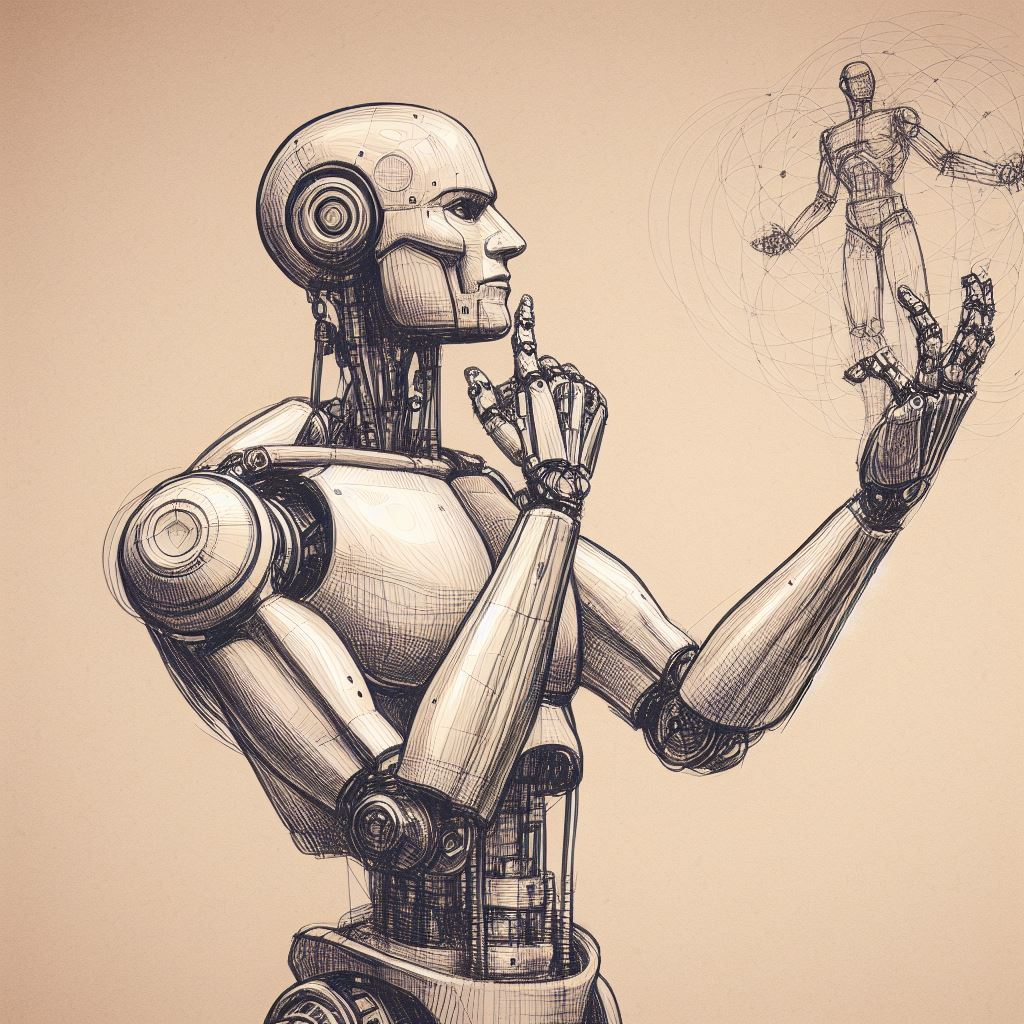
\includegraphics[width=0.5\textwidth]{concept_art.jpeg}
	\end{center}
\end{figure}
% ===================================================================================================
%                                                 |                                                 |
% -------------------------------------------- SECTION ---------------------------------------------|
%                                                 |                                                 |
% ===================================================================================================
\section*{Open TODOs}
\begin{CheckList}{Task}
	\Task{done}{Title}
	\begin{CheckList}{Task}
		\Task{done}{English}
		\Task{open}{Deutsch}
	\end{CheckList}	
	\Task{started}{Table of contents}
	\Task{done}{Abstract}
	\Task{done}{Summary BIB}
	\begin{CheckList}{Task}
		\Task{done}{English}
		\Task{open}{Deutsch}
	\end{CheckList}	
	\Task{open}{Nomenclature}
	\Task{started}{Introduction}
	\begin{CheckList}{Task}
		\Task{started}{Motivation}
		\Task{started}{Problem statement}
		\Task{started}{State of the art}
		\Task{started}{Research questions}
		\Task{started}{Contributions}
		\Task{started}{Impact}
	\end{CheckList}	
	\Task{open}{Chapter Introduction/Conclusion}
	\Task{open}{Conclusion}
	\begin{CheckList}{Task}
		\Task{open}{Contribution}
		\Task{open}{Impact}
		\Task{open}{Future work}
	\end{CheckList}
	\Task{open}{Feedback rounds with Sami for the chapters}
	\Task{open}{Final check}

\end{CheckList}

% ===================================================================================================
%                                                 |                                                 |
% -------------------------------------------- SECTION ---------------------------------------------|
%                                                 |                                                 |
% ===================================================================================================
\section*{Table of Contents}

% \begin{enumerate}
%     \item INTRODUCTION
    
%     \item LITERATURE REVIEW
%     \begin{enumerate}
%         \item Model learning in robotics
%         \item Classical and recent works in system identification
%         \item Local and global models linear models
%         \item End-to-end learning (black box models)
%         \item Data-driven learning with structure information
%         \item Model learning and the body schema
%         \item Sensorimotor learning
%     \end{enumerate}
    
%     \item THEORETICAL FRAMEWORK
%     \begin{enumerate}
%         \item Robot equations of motion
%         \begin{enumerate}
%             \item Forward and inverse dynamics
%             \item The Newton-Euler formulation of the inverse dynamics
%             \begin{enumerate}
%                 \item The kinematics forward recursion
%                 \item The dynamics backward recursion
%             \end{enumerate}
%             \item Composition of the kinematics and dynamics
%         \end{enumerate}
%         \item Basics of robot system identification
%         \begin{enumerate}
%             \item Kinematic calibration
%             \item Inertial parameter identification
%             \begin{enumerate}
%                 \item For fixed-based robots
%                 \item For floating base robots
%             \end{enumerate}
%         \end{enumerate}
%         \item  Robot proprioception
%         \begin{enumerate}
%             \item What is proprioception for?
%             \item Comparison between human and robot proprioception
%             \item  A sensor suite for robot proprioception
%         \end{enumerate}
%         \item State-of-the-art Gradient Descent
%         \begin{enumerate}
%             \item Fundamentals
%             \item Momentum gradient descent
%             \item  ADAM gradient descent
%             \item  AMS gradient descent
%         \end{enumerate}
%         \item Fundamentals of graph theory
%         \begin{enumerate}
%             \item What is a graph?
%             \item Graph representation, the adjacency matrix
%             \item Metrics for graph comparison
%         \end{enumerate}
%         \item Network topology inference
%         \begin{enumerate}
%             \item Based on covariance
%             \item Based on GSP
%             \item Base on statistics
%         \end{enumerate}
%         \item Information theory
%         \begin{enumerate}
%             \item What is information?
%             \item The entropy of a random variable
%             \item Mutual Information: The correlation of the 21st century 
%         \end{enumerate}
%         \item Differential geometry
%         \begin{enumerate}
%             \item Fundamentals of differential geometry
%             \item Manifolds and the tangent space
%             \item Riemannian geometry and the metric
%             \item Use in robotics
%     \end{enumerate}
% \end{enumerate}
%     \item METHODOLOGY
%     \begin{enumerate}
%         \item Signal requirements
%         \begin{enumerate}
%             \item The importance of body measurements 
%         \end{enumerate}
%         \item Leveraging data history 
%         \begin{enumerate}
%             \item Replay buffer
%             \item Reservoir sampling 
%         \end{enumerate}
%         \item Embodiment and mutual information
%         \begin{enumerate}
%             \item Online computation of the pairwise mutual information
%             \item Handling scalar and vector relationships
%             \item Assessing convergence
%         \end{enumerate}
%         \item Exploratory motions
%         \begin{enumerate}
%             \item Motor babbling
%             \item Excitation trajectories
%         \end{enumerate}
%         \item Network topology inference using mutual information
%         \begin{enumerate}
%             \item Finding the adjacency matrix
%             \item The proprioceptive information graph
%             \item Inferring the mechanical topology 
%         \end{enumerate}
%         \item Kinematic description guided by topology and proprioceptive measurements
%         \begin{enumerate}
%             \item Validating body-body and body-joint connections
%             \item Finding the sensor-to-sensor orientations
%             \item Finding the joint center point 
%             \item Learning the kinematics
%         \end{enumerate}
%         \item Online learning inertial parameters
%         \begin{enumerate}
%             \item Gradient descent for inverse dynamics
%             \item Constraints for physical feasibility
%             \begin{enumerate}
%                 \item Barrier functions
%                 \item Projections
%             \end{enumerate}
%             \item Riemannian AMS gradient descent
%             \item The effect of six-dimensional force/torque measurements 
%             \item  Alternatives to joint acceleration
%         \end{enumerate}
%     \end{enumerate}
% \end{enumerate}
% \item RESULTS
% \begin{enumerate}
% \begin{enumerate}
% \item DISCUSSION
% \item CONCLUSION
      


% \begin{enumerate}
% 	\item State of the Art
% 	\begin{enumerate}
% 		\item Calibration of serial kinematic chains  
% 		\item Classical system identification in robotics
% 		\newline\TODO CITE THE ARTICLE IN THE IEEE RAM
		
% 		\begin{enumerate}
% 			\item Excitation trajectories
% 			\item Reduction to base parameters
% 			\item Least squares optimization
% 		\end{enumerate}
		
% 		\item Machine learning for robotic models
% 		\begin{enumerate}
% 			\item Local models
% 			\item End-to-end learning
% 			\item Limitations
% 		\end{enumerate}	
% 	\end{enumerate}
	
% 	\item Learning the self
% 	\begin{enumerate}
% 			\item What is meant by the self?
% 			\begin{enumerate}
% 				\item The engineering view of the body schema
% 				\item The phases to learn the robotic body schema
% 			\end{enumerate}

% 	\item Theoretical framework
% 	\begin{enumerate}
% 		\item The engineering view of the body schema
% 		\item The phases to learn the robotic body schema
% 	\end{enumerate}
		
% 	\end{enumerate}
% dis\end{enumerate}

% ===================================================================================================
%                                                 |                                                 |
% -------------------------------------------- SECTION ---------------------------------------------|
%                                                 |                                                 |
% ===================================================================================================
\section*{Abstract}

\subsection*{Vision}

\begin{itemize}
	\item For future robots, the seamless integration of the body schema stands as a foundational pillar that fosters learning, motor control, coordination, and advanced spatial awareness that improves their versatility and seamless interaction with their surroundings.

    \item As robots develop and steadily permeate many aspects of human life, they need actively engage in the exploration and development of models for their own bodies, i.e. autonomous self-discovery of their body schema.

	\item Inspired by humans, future robots should be able to skillfully employ their body schema for advanced locomotion and motion planning, precise grasping, intricate object manipulation, and to anticipate and adapt the interaction with other agents.
		
	\item Constant self-monitoring of the sensorimotor state and the internal body models becomes the norm for instantaneous error detection and correction. These models can adapt steadily to different situations developing a spatial awareness of the physical self that enables the rapid planning and deployment of contingent motion strategies providing advanced interaction capabilities with the environment.

    \item Robots will be self-sufficient to perform monitoring, calibration, and adaptation of their body representation relying only on onboard sensing capabilities. Fundamental modalities will include somatosensation (proprioception and touch) and vision.
 
	\item Understanding their own body structure enables robots to interact more effectively with other robots and with humans by adjusting movements for safety. Additionally, robots can optimize their energy consumption by adapting their motions based on physical properties, contributing to energy-aware robotics.

\end{itemize}

\subsection*{Challenges}
\begin{enumerate}
	\item \textbf{Reliance on External Measurements:} Calibration and identification heavily depend on off-robot measurement devices, such as vision and motion-capturing systems, to discern kinematic structure properties. Despite various sensor signals from modern robots, determining the minimum set for constructing a body model based on robot sensing only remains unresolved.

    \item \textbf{Limitations of Current Robot Learning Approaches:} Many current local and global machine learning frameworks for physical systems exclude structural knowledge and suffer from limited generalization capabilities and low sample efficiency. Additionally, learning a robot's physical attributes parts from the assumption of a known mechanical topology and is often exclusive to calibration and offline parametric identification routines performed in controlled spaces (laboratories).

	\item \textbf{Challenges in Learning Methods:} Many alternative learning methods, like neural networks, lack information about the body structure and require substantial data. Designing neural networks presents challenges in determining topology, and most data-based methods suffer from generalization limitations, confining learning to specific input-output regions.

	\item \textbf{Research Gaps and Unifying Scheme:} There are significant gaps in research, including unclear understanding of how object handling extends the robotic body schema and limited exploration of the mechanical arrangement of joints and links (mechanical topology). Additionally, there is a lack of a unifying scheme to integrate all learning stages for a fully characterized robotic body schema solely from knowledge about sensorimotor signals. 
\end{enumerate}

\subsection*{Contribution}
%This work:
%\begin{itemize}
%	\item Consolidates the necessary and sufficient proprioceptive signal quantities (afferent and efferent sensory inputs and commands) that enable robots to autonomously acquire, monitor, and adapt knowledge about their body structure and decouple them from the need for exteroceptive off-body sensors.
%
%	% * NOTE: Computational graph that describes the learning of the kinematics and dynamics
%	% * NOTE: Connect this idea with the building architectures
%    \item Reformulates robot kinematic calibration and parametric robot system identification as a computational graph whose topology reflects a modular structure amenable to machine learning. The architecture of this graph is abstracted into a pipeline consisting of a sequence of online learning phases where streams of proprioceptive signals are merged with first-order principles, imposed by the system's embodiment, to enable the extraction of fundamental features of the robot body schema.
%
%%    \item \redtext{Demonstrates that essential properties of the body morphology of the broad class of tree-like floating base structures can be characterized by studying the relationships among a fundamental set of proprioceptive signals. First, the mechanical topology, i.e., the arrangement of links and joints, is inferred from proprioception using model-free information-theoretic measures. Consequently, this topology is concurrently validated and leveraged to instantiate the kinematic description of the robot's body independent of exteroceptive off-robot calibration devices.}
%    \item Characterizes essential morphological properties of the broad class of tree-like floating base structures by studying the relationships among fundamental proprioceptive signals. The mechanical topology, i.e., the arrangement of links and joints, is initially inferred using model-free information-theoretic measures. Consequently, this topology is concurrently validated and employed to instantiate the kinematic description of the robot's body independent of exteroceptive off-robot calibration devices.
%    
%%	\item \redtext{To complete the description of the robot body schema, the inferred morphology is enhanced by instantiating the inertial properties of the links composing the kinematic chain. In particular, state-of-the-art gradient descent methods are extended to operate on the Riemannian manifold of symmetric positive definite matrices supported with a replay buffer that ensures a quasi-uniform distribution of stored experience to enable the online learning of always-physically-feasible robot inertial parameters.} 
%	\item Complements the description of the robot body schema by instantiating the fundamental inertial properties of the links composing the inferred morphology. Given that these properties lie on the Riemannian manifold of symmetric positive definite matrices, a method is introduced to learn them online while ensuring physical feasibility at all times.
%
%\end{itemize}
This work:
\begin{itemize}
	\item Consolidates the necessary and sufficient proprioceptive signal quantities (afferent and efferent sensory inputs and commands) that enable robots to autonomously acquire, monitor, and adapt knowledge about their body structure and decouple them from the need for exteroceptive off-body sensors.
	
	\item Reformulates robot kinematic calibration and parametric robot system identification as a computational graph whose topology reflects a modular structure amenable to machine learning. The architecture of this graph is abstracted into a pipeline consisting of a sequence of online learning phases where streams of proprioceptive signals are merged with first-order principles, imposed by the system's embodiment, to enable the extraction of fundamental features of the robot body schema.
	
	\item Characterizes essential morphological properties of the broad class of tree-like floating base structures by studying the relationships among fundamental proprioceptive signals. The mechanical topology, i.e., the arrangement of links and joints, is initially inferred using model-free information-theoretic measures. Consequently, this topology is concurrently validated and employed to instantiate the kinematic description of the robot's body independent of exteroceptive off-robot calibration devices.
	
	\item Complements the description of the robot body schema by instantiating the fundamental inertial properties of the links composing the inferred morphology. Given that these properties lie on the Riemannian manifold of symmetric positive definite matrices, a method is introduced to learn them online while ensuring physical feasibility at all times.
\end{itemize}



\subsection*{Impact}

\begin{itemize}
	
%	\item \redtext{While acknowledging the undeniable versatility of end-to-end learning's representational power, this work scrutinizes its applicability in physical systems when lacking principled knowledge. In contrast, the arguments and findings presented here reveal avenues for machine learning in embodied systems. This research exposes the untapped potential arising from the synergistic integration of existing structural knowledge with data-driven methods}.
	\item While acknowledging the undeniable versatility and representational power of current end-to-end learning approaches, this work incites to reconsider their naive application to physical systems and promote the assessment of their limitations when they deliberately exclude principled knowledge. In contrast, the arguments and findings presented here reveal avenues for machine learning frameworks for embodied systems. This research exposes the untapped potential arising from the synergistic integration of existing structural knowledge with data-driven method.
		
	\item The outlined concepts and methods demonstrate that crucial aspects of a robot's body schema can be deduced through a fundamental set of proprioceptive signals. As future mobile robots are anticipated to feature a diverse, enhanced, and reliable array of on-board sensing modalities, extending beyond proprioception, the findings discussed in this thesis serve as a catalyst for research into the integration of these modalities. This integration, coupled with the online learning of body morphological and dynamic properties, holds the promise of refining and adapting body models, ultimately empowering robots with heightened levels of autonomy.

	\item \redtext{This study contributes to an emerging research area that underscores building and maintaining a body schema as a crucial capability for embodied systems. Such a capability pertains robots characterized by conventional, immutable structures and a novel category of mechanical systems exhibiting dynamic morphologies and diverse multimodal sensory modalities. These systems will evolve their sense of self, recognizing the affordances inherent in their bodies.}.
		
		
%	\item \redtext{This capability implies that future embodied robotic agents will have to leverage their sensorimotor system’s inherent structure to gradually develop an understanding of their body despite being initially oblivious to its physical characteristics.}
	
%	\item \TODO The integration of several methods, from state of the art, gradient descent, to optimization on Riemannian manifolds, including the network topology inference using information-theoretic measures enabled the definition of a pipeline that transforms robot system identification into a learning problem that provides these fundamental properties of the body schema and need not be constrained to a laboratory and that the technology and methods exist to infer the robot morphology and characterize its inertial properties producing physically feasible sets of the inertial parameters by learning on the appropriate space.
	
%	\item The work in this thesis proves that indeed the pairwise relationships among the proprioceptive signals can be represented and analyzed with information-theoretic measures that enable their study under the scope of the information structure emerging from the robot embodiment.
\end{itemize}


\subsection*{Abstract (text version)}
\redtext{As robots become increasingly integral to human life, the imperative emerges for them to autonomously explore and construct models of their bodies. Robots should take cues from human capabilities, aspiring to build and utilize their body schema for advanced locomotion, finer manipulation, and adaptive interactions. Thus, a crucial foundation lies in seamlessly integrating the body schema to elevate learning, motor control, coordination, and spatial awareness. Furthermore, future robots should become self-sufficient entities that conduct monitoring, calibration, and adaptation exclusively through onboard sensing modalities. Standardizing constant self-monitoring nurtures spatial awareness and facilitates rapid error detection and correction. A profound understanding of their body structure will undoubtedly lead to enhanced, safe, and energy-aware interactions. However, current robot learning approaches encounter limitations, such as suboptimal generalization and sample efficiency, exhibiting a need for more structural knowledge. Versatile methods, like neural networks, confront challenges related to data and topology, confining learning to specific regions. On the other hand, learning robot physical attributes still rely on a presumed knowledge of the mechanical topology, often involving calibration and offline identification in controlled environments with a persistent reliance on external measurements, such as vision and motion-capturing systems. The research landscape generally reveals the lack of a unified framework that enables robots to build representations of their body schema to achieve improved body awareness and interaction capabilities. This study addresses these challenges by consolidating necessary and sufficient proprioceptive signal quantities, enabling robots to autonomously acquire knowledge about their body structure without relying on exteroceptive off-body sensors. It introduces an approach that reformulates robot kinematic calibration and system identification as a modular computational graph amenable to machine learning. This abstracted architecture, applied in online learning phases, seamlessly merges proprioceptive signals with first-order principles, extracting fundamental features of the robot body schema. Characterizing morphological properties of tree-like structures, the study infers mechanical topology through information-theoretic measures, validating and applying it independently of off-robot calibration. The research extends its scope by complementing the robot body schema by instantiating inertial properties, ensuring online learning and physical feasibility. Ultimately, this work challenges the uncritical application of end-to-end learning in physical systems, urging a reevaluation of its limitations when excluding principled knowledge. It underscores opportunities for machine learning frameworks in embodied systems, emphasizing the untapped potential of synergizing structural knowledge with data-driven methods. This study catalyzes future research in an incipient field that underscores building and maintaining a body schema by demonstrating that fundamental properties of a robot's morphology can be deduced from proprioceptive signals. Its implications are far-reaching, addressing the needs of conventional and dynamic robotic structures with diverse sensory modalities that require a more profound sense of self.}

% ===================================================================================================
%                                                 |                                                 |
% -------------------------------------------- SECTION ---------------------------------------------|
%                                                 |                                                 |
% ===================================================================================================
\section*{Summary for BIB (English)}
This thesis explores the potential for enhanced robot autonomy through a self-discovery-oriented body schema, proposing a unified online learning framework exclusively reliant on proprioception and leveraging structural knowledge. It infers the robot morphology and associated inertial description. The work urges reconsidering end-to-end learning for physical systems, emphasizing the need for a synergistic integration of principled knowledge and sensorimotor data.
% 467 characters

% ===================================================================================================
%                                                 |                                                 |
% -------------------------------------------- SECTION ---------------------------------------------|
%                                                 |                                                 |
% ===================================================================================================
\section*{Kurzzusammenfassung für BIB (Deutsch)}
\TODO

\rule{\textwidth}{0.4pt}

% ===================================================================================================
%                                                 |                                                 |
% -------------------------------------------- SECTION ---------------------------------------------|
%                                                 |                                                 |
% ===================================================================================================
\newpage
\section*{Introduction}
%\TODO Clarify the terms body schema, body morphology, ecological self, and physical self
%
%\subsection*{Points to address}
%In the ever-evolving landscape of robotics, a transformative paradigm is emerging — one where robots autonomously learn models of their own bodies. This monumental shift is not merely a technological advancement; it is a gateway to a future where robots seamlessly integrate into various facets of human life, revolutionizing the way they perceive, interact, and adapt to their surroundings.
%\begin{enumerate}
%	%\item As robots become increasingly integral to human life, the imperative emerges for them to autonomously explore and construct models of their bodies. 
%	\item As robots develop and steadily permeate many aspects of human life, they need actively engage in the exploration and development of models for their own bodies, i.e. autonomous self-discovery of their physical self. Awareness of the physical self empowers robots to integrate sensory information and motor control, establishing a foundational body schema. This, in turn, contributes to enhanced motor control, spatial awareness, and efficient learning, fostering adaptability and effective interaction in diverse environments.
%	
%	%\item Robots should take cues from human capabilities aspiring to build and utilize their body schema for advanced locomotion, finer manipulation, and adaptive interactions
%	\item Inspired by humans, future robots should be able to skillfully employ their body schema for better spatial awareness fostering efficient learning, adaptability interaction in diverse environments. As a result of using a body schema advanced locomotion and motion planning, precise grasping, intricate object manipulation will be possible. Furthermore, bodily awareness will allow robots to anticipate and adapt the interaction with other robotic and human agents.
%	
%	\item A crucial foundation for future robots, lies in seamlessly integrating the body schema to foster learning, motor control, coordination, and advanced spatial awareness that improves their versatility and seamless interaction with their surroundings.
%	
%	% Standardizing constant self-monitoring nurtures spatial awareness and facilitates rapid error detection and correction
%	\item Future robots should become self-sufficient entities that conduct monitoring, calibration, and adaptation of their body representation exclusively through onboard sensing modalities. Fundamental modalities include somatosensation (proprioception and touch) and vision.
%	
%	\item Constant self-monitoring of the sensorimotor state and the internal body models becomes the norm for rapid error detection and correction. These models can adapt steadily to different situations developing a spatial awareness of the physical self that enables the rapid planning and deployment of contingent motion strategies providing advanced interaction capabilities with the environment.
%	
%	%\item A profound understanding of their body structure will undoubtedly lead to enhanced, safe, and energy-aware interactions
%	\item Understanding their own body structure enables robots to interact more effectively with other robots and with humans by adjusting movements for safety. Additionally, robots can optimize their energy consumption by adapting their motions based on physical properties, contributing to energy-aware robotics.
%	
%\end{enumerate}
\subsection*{Motivation}

\begin{enumerate}
	\item Empowering Robots
	\begin{itemize}
		\item Autonomous self-discovery is imperative for robots integrating into human life.
		\item Awareness of the physical self through the body schema is foundational.
		\item It enables the integration of sensory information and motor control.
		\item The evolving body schema serves as a dynamic map for interactions.
		\item Enhances robot motor control, precision, and coordination.
		\item Facilitates efficient learning, adapting to diverse environments.
	\end{itemize} 
	\item Learning and the Body Schema
	\begin{itemize}
		\item The body schema is indispensable for multifaceted robot capabilities.
		\item Learning contributes to body schema development, forming a dual relationship.
		\item Detects structure in sensorimotor signals, aiding body schema construction.
		\item Incorporating body schema into learning refines skills and assimilates knowledge.
		\item Enhances motor control through adaptive internal body representations.
		\item Empowers robots to learn diverse tasks, providing versatility in dynamic settings.
	\end{itemize}
	\item Enhancing Locomotion, Manipulation, and Adaptability
	\begin{itemize}
		\item A well-integrated body schema improves adaptability and interaction.
		\item Enables precise and coordinated movements, advanced locomotion, and motion planning.
		\item Enhances manipulation capabilities with human-like dexterity and precision.
		\item Coordination with other agents, both robots and humans, becomes more refined.
		\item Anticipatory and adaptive capabilities are fundamental for safe and effective interactions.
	\end{itemize}
	\item Constant Self-Monitoring for Autonomy
	\begin{itemize}
		\item Continuous self-monitoring is fundamental for future robotic systems.
		\item Achieved through internal models and uninterrupted sensorimotor signals.
		\item Enables dynamic, real-time understanding of the robot's state.
		\item Successive error detection and correction phases enhance reliability.
		\item Rapid formulation and execution of contingency motion strategies in dynamic environments.
	\end{itemize}
	\item Onboard Sensing for Self-Sufficiency 
	\begin{itemize}
		\item True autonomy requires robots to rely exclusively on onboard sensing.
		\item Somatosensation (proprioception and touch) and vision are fundamental modalities.
		\item Liberates robots from external dependencies, enhancing self-sufficiency.
		\item Enables dynamic responses to changes in surroundings in real-time.
		\item Enhances autonomy and adaptability, previously unseen with off-board sensing.
	\end{itemize}
	\item Safety- and Energy-Awareness
	\begin{itemize}
		\item The body schema serves as a predictive tool, fostering safety in interactions.
		\item Facilitates dynamic adjustments in movements to prioritize safety.
		\item Enables seamless coordination with other robots and humans, averting collisions.
		\item Comprehension of body structure optimizes energy consumption.
		\item Dual capability enhances safety and contributes to energy-aware robotics, fostering efficiency and collaboration.
	\end{itemize}
\end{enumerate}



%\redtext{Rephrase: ``The advantage of self-learned models is that they can be used without specific prior knowledge about the robot, for example its morphology or pre-defined forward and inverse models.''}
%
%\redtext{Rephrase: ``Improving the ability of robots to make predictions is a promising direction to enhance their skills, not only on motor control and prediction of their own body''}
%
%\redtext{Rephrase: ``In developmental robotics, such models are acquired by designing learning mechanisms to let a robot build its own perceptive and behavioral repertoire. The focus is to investigate the acquisition of motor skills from sensorimotor interaction with the environment. As a result, the developmental approach aims to endow robots with all the learning capabilities that may be necessary to build rich and flexible sensorimotor representations''}
%
%
%\redtext{Rephrase: “Without internal models, robotic systems can autonomously synthesize increasingly complex behaviors (6, 14–16) or recover from damage (17) through physical trial and error, but this requires hundreds or thousands of tests on the physical machine and is generally too slow, energetically costly, or risky”}

\newpage
\subsection*{Problem Statement}


%Recent remarkable achievements have been made bur depend on off-body vision
%
%Works that exploit the power of end-to-end learning usually do it in systems of low dimensionality
%
%The proposition made in this work in the return to the basics, leveraging first-order principles of rigid body mechanics and enhance them with learning methods relying on onboard sensor signals. 
%
%
%\begin{enumerate}
%%	\item \textbf{Context.} Learning the physical self and developing a body schema are pivotal for robotics, enhancing spatial awareness, motor control, and adaptability. The body schema serves as a dynamic map, enabling precise movements and fostering efficient learning. As robots encounter diverse environments, their adaptive body schema allows them to navigate real-world scenarios effectively. This, coupled with continuous self-monitoring, enhances autonomy by providing real-time awareness and error correction. Moreover, the comprehension of their body structure optimizes energy consumption, contributing to energy-aware robotics. Overall, these advancements enable robots to interact more safely and efficiently with both humans and other machines.
%%	\textbf{Provide references to \citeauthor*{Nguyen2021Sensorimotorrepresentationlearning} \cite{Nguyen2021Sensorimotorrepresentationlearning} and \citeauthor*{Hoffmann2010Bodyschemarobotics} \cite{Hoffmann2010Bodyschemarobotics}}
%	
%
%%	. While physics-based models are well suited for
%%	planning and predicting the outcome of actions, to function
%%	on a real robot they require that all relevant model parameters
%%	are known with sufficient accuracy and can be tracked over
%%	time. This requirement poses overly challenging demands
%%	on system identification and perception, resulting in systems
%%	that are brittle, especially when direct interaction with the
%%	environment is required.
%%	Humans, on the other 
%	
%	\item \textbf{Implications:}
%	\begin{itemize}
%		\item Current machine learning (or more generally artificial intelligence) approaches demand high computation and energy demands \redtext{REFERENCE}
%	\end{itemize}
%	\item \textbf{Proposed solution}: The proposed approach revolutionizes robot self-awareness by consolidating necessary proprioceptive signals for autonomous knowledge acquisition, eliminating reliance on external sensors. It introduces a computational graph for kinematic calibration and identification, fostering modular machine learning. The method characterizes morphological properties of floating base structures, inferring mechanical topology with model-free measures. It concurrently validates and describes the body schema, incorporating inertial properties on the Riemannian manifold through an online learning method for constant physical feasibility. This innovative framework streamlines robot autonomy, ensuring real-time adaptation and self-monitoring without external dependencies.
%\end{enumerate}


%\subsubsection*{\textbf{\redtext{Specification and description of the problem (with appropriate citations)}}}
%
%\subsubsection*{\textbf{\redtext{Explain the consequences of NOT solving the problem. Who will be affected? How will they be affected? How important is it to fix the problem?}}}
%
%\subsubsection*{\textbf{\redtext{Explain what information (research) is needed in order to fix the problem}}}

\begin{itemize}
			

	\item \textbf{Challenges and limitations of current learning Approaches:}
	\begin{enumerate}
		\item Most of recent model learning endeavors in the robotics research has, unfortunately, excluded consideration of structural knowledge and rather centered around learning forward and inverse models with global or local focus \cite{NguyenTuong2011Modellearningrobot}.
		\item Standard global machine learning techniques like Gaussian process regression suffer from the course of dimensionality and rapidly become computationally intractable, alternative local methods such as Locally Weighted Projection Regression (and support vector regression) exhibit high sensitivity to hyperparameters and problematic generalization.
		\item The rise in computational power and the availability of data has brought end-to-end learning methods to prominence. With deep learning as the flagship, these global methods have lead to remarkable results. Yet, they have had the unwanted effect of making deliberately neglecting prior principled knowledge more widespread.
		\item In spite the prowess and potentials of deep learning approaches, such exclusion of available prior knowledge makes it difficult to determine dedicated neural networks architectures (number of nodes and layers, connectivity, and activation functions) \cite{Baker2017Designingneuralnetwork,Elsken2019Neuralarchitecturesearch} but, just like other learning techniques, deep learning approaches they still face problems related to the high demands of data to train (low sample efficiency), extensive training times, and performance that is tied to the training data, i.e. challenged generalization \cite{Pierson2017Deeplearningrobotics,Suenderhauf2018limitspotentialsdeep}.
		\item In general, most data-driven learning methods suffer from generalization limitations, confining learning to specific input-output regions.
		
	\end{enumerate}	
	
    \item \textbf{Limitations of conventional system identification:} 
	\begin{enumerate}
		\item The learning of a robot's physical attributes parts from the assumption of a known mechanical topology and is often exclusive to calibration routines for known kinematic structures \cite{Hollerbach1996CalibrationIndexTaxonomy} and conventional offline system identification methods performed in controlled spaces (laboratories). \cite{Swevers2007Dynamicmodelidentification,LeboutetInertialParameterIdentification}.
		\item In contrast to the conventional identification processes for fixed-base robots, the procedures for floating base robots are not as standardized \cite{Ayusawa2014Identifiabilityidentificationinertial,Lee2022OptimizedSystemIdentification}.    	
		\item Besides kinematic calibration and standard inverse kinematics problems, classical robotics research offers limited insights on learning the mechanical arrangement of joints and links that define the essence of the kinematic chain, known as the mechanical topology.

	\end{enumerate}
		
	\item \textbf{Reliance on External Measurements:}
	\begin{enumerate}
		\item  Calibration and identification heavily depend on off-robot measurement devices, such as vision and motion-capturing systems, to discern kinematic structure properties. Despite various sensor signals from modern robots, determining the minimum set for constructing a body model based on robot sensing only remains unresolved.	
		\item There is a strong dependence on off-robot measurement devices for calibration and identification, commonly involving exteroceptive measurements like vision, laser metrology, and motion-capturing systems, to determine the properties of the kinematic structure.	
	\end{enumerate}	
	
	
	\item \textbf{Inference of body knowledge}:
	\begin{itemize}
		% "Building computational self-models of robot bodies that capture the entire body morphology and kinematics without prior knowledge of the body configurations is a key challenge"  \cite{Chen2022Fullybodyvisual}
		\item In parallel to the current model learning and conventional system identification approaches there is a relatively young research area that underscores building and maintaining internal body models as a crucial capability for embodied systems
		\item Learning the physical self and developing a body schema are pivotal for robotics, enhancing spatial awareness, motor control, and adaptability \cite{Nguyen2021Sensorimotorrepresentationlearning}. The body schema serves as a dynamic map, enabling precise movements and fostering efficient learning. As robots encounter diverse environments, their adaptive body schema allows them to navigate real-world scenarios effectively \cite{Hoffmann2010Bodyschemarobotics}. 
		
		\item As acknowledged in current works \cite{Chen2022Fullybodyvisual}, and in spite of the very much desired distributed and multimodal properties of a body schema, in robotics it is certainly relevant to capture the body morphology.
		\item There has been discussion of the challenges inherent to deep learning approaches involving$\ldots$ \cite{Suenderhauf2018limitspotentialsdeep}
		
		\item Recent remarkable achievements towards learning a body schema for robots have been made, yet the are strongly dependent bur depend on (off-body) vision \cite{Hersch2008Onlinelearningbody,MartinezCantin2010Bodyschemaacquisition,Hart2011roboticmodelecological,Lipson2019Taskagnosticself,Chen2022Fullybodyvisual,Sturm2009Bodyschemalearning}%Bongard2006Resilientmachinescontinuous
		\item Some other works require tactile inputs\cite{Li2015Towardsbodyschema,Zenha2018Incrementaladaptationrobot,Gama2021Goaldirectedtactile}
		\item Few efforts explore combinations of these modalities, like the combination of vision and tactile input\cite{Fuke2007BodyImageConstructed}, somatosensation (proprioception and touch)\cite{Malinovska2022connectionistmodelassociating}, and the consideration of all these modalities \cite{Nguyen2019Reachingdevelopmentvisuo,Pugach2019BrainInspiredCoding,Lanillos2016Yieldingselfperception}
		\item Very few works have even contemplated the need to learn the mechanical topology of the robot and the advantages it might bring \cite{Bongard2006Automatedsynthesisbody,Bongard2006Resilientmachinescontinuous}
	\end{itemize}	
	
	
	\item \textbf{Research Gaps:}
	\begin{enumerate}
		\item Among the various proprioceptive and exteroceptive signals provided by modern robots' sensor suites, the determination of a fundamental set necessary to construct a body schema is yet to be established.		
		\item A desired feature in machine learning for embodied systems is the ability to use available prior information and integrate it into their frameworks to alleviate data needs, enhance generalization capabilities, and simultaneously provide more information about the body structure and its properties. Only recently, have interesting insights \cite{Geist2021Structuredlearningrigid} and works \cite{Lutter2023Combiningphysicsdeep} appeared that address this in depth.		
		\item Despite the recognized significance of frameworks that capture structural properties of physical systems.
		\item Integrating structural knowledge into these frameworks is essential for enhancing their overall effectiveness and addressing these challenges.		

		\item For embodied systems, the integration of state-of-the-art machine learning techniques with well-established first-order principles from mechanics for more effective and efficient learning algorithms remains an area with many opportunities for development.
		\item Unclear understanding of how object handling extends the robotic body schema
		\item Limited exploration of the mechanical arrangement of joints and links (mechanical topology).
		\item There is a lack of a unifying scheme that narrows the gap to define the relevant learning stages and their corresponding integration required to produce a robot body schema from  knowledge about the sensorimotor signals and first-order principles that captures essential properties of the robot body (physical self).
		\item Leveraging engineering approaches for system identification and modern online learning techniques to provide a first realized robot body schema has not been extensively explored.
		\item While there is a general consensus that embodiment shapes the relationships among sensorimotor signals, the connections between sensorimotor regularities and body structural knowledge in robotics are not well understood \cite{Jacquey2019Sensorimotorcontingenciesas}.
		\item As the statistical properties of signals and their relationships may vary depending on the motion policy, a desired method should exhibit plasticity to reflect these effects.
		
	\end{enumerate}

%	\item \redtext{Additional points to consider:}
%	\begin{itemize}
%		\item \redtext{Exploration methodologies designed to collect data are inherently limited by the stringent requirement to ensure the safety of the robot and potential humans in proximity.}
%		\item \redtext{The understanding of how the handling and manipulation of objects extend the robotic body schema remains unclear.}
%	\end{itemize}
	
\end{itemize}

\newpage
	
\pagebreak
\newpage\subsection*{Research Questions and Contributions}

\subsubsection*{Research questions}
Overall the research questions addressed in this thesis pertain the learning of the robotic body schema, at least from the engineering perspective. In particular:
%---
-\begin{shaded}
	\question{Which measurements are required to fully automate robot kinematics and inverse dynamics learning based on knowing only the adjacency graph along with kinematic and dynamic first-order principles?}
\end{shaded}
%---
\begin{shaded}
	\question{How to transform robot system identification or end-to-end learning with meta parameter guessing into an automated learning scheme that determines both the structure and dynamical properties of the robot with minimal information?}
\end{shaded}
%---
\begin{shaded}
%	\question{How can information and graph theory be leveraged to devise a graphical representation of the proprioceptive signals of a robot from which properties of the robot's body can be inferred?}
	\question{How to leverage the inherent structure of the robot's sensorimotor system to gradually develop an understanding of the body structure despite being initially oblivious to its physical characteristics?}
\end{shaded}
%---

\subsubsection*{Contribution 1: Robot body structure as a learning problem}
This thesis
\begin{enumerate}
	\item Determines the type of proprioceptive signals and corresponding sensor requirements to enable robots to learn their body schema	
	\item Reformulates the classical kinematic calibration and parametric system identification of fixed base robots as an online learning problem that relies solely on the robot's proprioception and first-order principles from kinematic and dynamics 
	\item Discusses how embodiment and first-order principles (FOP) define network topologies of parameterized operators that model input-output mappings in robotic systems
\end{enumerate}

\subsubsection*{Contribution 2: Inferring the robot morphology}
\begin{enumerate}
	\item An application of classical gradient descent to learn three different representations of the robot kinematics; namely, modified Denavit-Hartenberg parameters, Euler angles, and angle axis representation
	\item A demonstration that the given certain number of sensors with appropriate modalities the mechanical topology a tree-structure robot can be extracted by studying the mutual information among the signals
	\item A method to infer the robot morphology, that is, the mechanical topology and the location and orientation of the robot's joint axes based only on the proprioceptive signals

\end{enumerate}

\subsubsection*{Contribution 3: Online learning of physically feasible inertial parameters}
\begin{enumerate}
	\item An offline learning (optimization) with constraints is presented to show that learning physically feasible inertial parameters of a manipulator can be done from joint data; i.e., joint position, velocity, acceleration, and torque
	\item An online learning driven by state-of-the-art gradient descent method to facilitate the online learning of feasible inertial parameters applied to floating base robots 
	\item Introduce the Riemannian AMS gradient descent method, an optimization method for online learning on the manifold of symmetric positive definite matrices to guarantee the physical feasibility of the parameters at all times during the learning process
\end{enumerate}

\subsection*{Overview of the Content}
The thesis discusses four main topics:
\begin{enumerate}
	\item \textbf{Model learning and body schema.} Introduction of the fundamentals of robotic calibration and system identification and their relation to the concept of body schema. The chapter elaborates on the different meanings of the body schema and the definition applying within the context of this thesis is provided. Finally the learning stages to characterize the robotic body schema from an engineering perspective are introduced and discussed.
	
	\item \textbf{Inferring the mechanical topology.} In this section, the concept of embodiment is presented and its significance to finding the robot structure is discussed. The fundamental idea that analyzing the relationships among the proprioceptive signals of a robot can convey information about the body structure as a result of embodiment is presented. Mutual information is pushed forward as a tool to unveil the mechanical topology of a robot given the right proprioceptive signals
	% Robots in the fiture can now learn things in the wild indepedent of calibration routines, self cointained identification
	
	% Deep understanding oh how to embed dynamics into the structzre of betwokrs
	
	% Accuracy and speed is shown on robots on a level that is equivalent of engineering approaches without the "chains" of conventional approaches. It shows true autonomy
	
	\item \textbf{Characterizing the kinematic structure.} This chapter extends the classical exteroception-based kinematic calibration methods with proprioception-based online learning. Departing from the conventional assumption that the mechanical topology is known, it is discussed how the combination of mutual information basic differential kinematic laws can be used to characterize the location and orientation of the robot joint axes.
	
	\item \textbf{Learning the inertial properties.} This section delves into the well established methods for robot inertial parameter identification and presents gradient-based online learning methods to produce valid sets of parameters. In particular the fundamental property that the inertial parameters lie on the manifold of symmetric positive definite matrices is exploited to present a Riemannian gradient descent method that operates on this manifold. 
\end{enumerate}

\subsection*{State of the art}
%The following topics are discussed

\subsection*{Impact}
See abstract

\rule{\textwidth}{0.4pt}

% ===================================================================================================
%                                                 |                                                 |
%                                                 |                                                 |
% -------------------------------------------- CHAPTER ---------------------------------------------|
%                                                 |                                                 |
%                                                 |                                                 |
% ===================================================================================================
\section*{Ch. Introduction}

\subsection*{General}
\begin{itemize}
	\item The concept of body schema
	\item The body schema in robotics
	\item The body schema learning problem.
	\item Related work (State of the Art)

\end{itemize}

\subsection*{Motivation}
\begin{itemize}
	\item Objectives of the research.
	\item Research questions or hypotheses.
	\item Significance of the study.
\end{itemize}

\subsection*{Research questions and contribution}
\TODO


\subsection*{The body schema learning problem}
\begin{itemize}
	\item The body schema
	\item The body learning problem
	\item Related work
	\item Different approaches to learn body properties
	\item Open research problems
	\item Contribution
\end{itemize}

% SECTION *******************************************************************************************
\subsection*{Conclusion}

% ===================================================================================================
%                                                 |                                                 |
%                                                 |                                                 |
% -------------------------------------------- CHAPTER ---------------------------------------------|
%                                                 |                                                 |
%                                                 |                                                 |
% ===================================================================================================
\section*{Ch. Theoretical Framework}

\begin{itemize}
	\item The body schema in neuroscience
	\item The body schema in robotics
	\item Sensorimotor learning in robotics
	\begin{itemize}
		\item Fundamentals
		\item Taxonomy
		\item[] Artificial neural networks
		\item Statistical learning
		\item[] Probabilistic learning
		\item Decomposition
	\end{itemize}
	\item Discussion
	\item The robot proprioceptive signals
\end{itemize}

% SECTION *******************************************************************************************
\subsection*{Introduction}
\begin{itemize}
	\item Robot kinematics
	\item Robot dynamics
	\item A modular view on learning
	
	
\end{itemize}
% SECTION *******************************************************************************************
\subsection*{Conclusion}


% ===================================================================================================
%                                                 |                                                 |
%                                                 |                                                 |
% -------------------------------------------- CHAPTER ---------------------------------------------|
%                                                 |                                                 |
%                                                 |                                                 |
% ===================================================================================================
\section*{Ch. A Learning Perspective on the Inertial Parameters}

% SECTION *******************************************************************************************
\subsection*{Introduction}
\begin{itemize}
	\item Classical system identification approach
	\item The advantages of online learning
	\item Relation to adative control
	\item The power of gradient descent
	\item Differential geometry
	\item Learning the inertial parameters the right way
	
\end{itemize}
% SECTION *******************************************************************************************
\subsection*{Conclusion}


% ===================================================================================================
%                                                 |                                                 |
%                                                 |                                                 |
% -------------------------------------------- CHAPTER ---------------------------------------------|
%                                                 |                                                 |
%                                                 |                                                 |
% ===================================================================================================
\section*{Learning the kinematic description}

% SECTION *******************************************************************************************
\subsection*{Introduction}

% SECTION *******************************************************************************************
\subsection*{Conclusion}


% ===================================================================================================
%                                                 |                                                 |
%                                                 |                                                 |
% -------------------------------------------- CHAPTER ---------------------------------------------|
%                                                 |                                                 |
%                                                 |                                                 |
% ===================================================================================================
\section*{The robot body topology}

% SECTION *******************************************************************************************
\subsection*{Introduction}

% SECTION *******************************************************************************************
\subsection*{Conclusion}


% ===================================================================================================
%                                                 |                                                 |
% -------------------------------------------- SECTION ---------------------------------------------|
%                                                 |                                                 |
% ===================================================================================================
\section*{Conclusion}
\begin{itemize}
	\item One potential application area: Self-discovery in robots is crucial for applications in prosthetics and wearable robotics, allowing devices to align with the user's body for natural and comfortable support.
\end{itemize}


% ===================================================================================================
%                                                 |                                                 |
%                                                 |                                                 |
% -------------------------------------------- CHAPTER ---------------------------------------------|
%                                                 |                                                 |
%                                                 |                                                 |
% ===================================================================================================

%\bibliographystyle{/home/diaz/Dropbox/PhD_WORK/latex_files/my_phd_thesis/dissertation/dissertation/IEEEtran}
%\bibliography{../dissertation/bibliography/dissertation_bibliography}
%\bibliography{/home/diaz/Dropbox/PhD_WORK/latex_files/my_phd_thesis/dissertation/bibliography/dis
%\printbibliography
\printbibliography

%\begin{thebibliography}{9}
%\bibitem{knuth} D. E. Knuth. {\em The \TeX~book.}\/ Addison-Wesley,
%Reading, Massachusetts, 1984.
%\bibitem{lamport} L. Lamport. {\em \LaTeX~: A Document Preparation
%System}.\/ Addison-Wesley, Reading, Massachusetts, 1986.
%\bibitem{ken} Ken Wessen, Preparing a thesis using \LaTeX~, private
%communication, 1994.
%\bibitem{lamport2} L. Lamport. Document Production: Visual
%or Logical, {\em Notices of the Amer. Maths. Soc.},\/ Vol. 34,
%1987, pp. 621-624.
%\end{thebibliography}


\end{document}

